\documentclass[journal,12pt,twocolumn]{IEEEtran}
\usepackage{setspace}
\usepackage{gensymb}
\singlespacing

\usepackage{graphicx}
%\usepackage{subfigure}

\usepackage[cmex10]{amsmath}
\usepackage{multicol}
\usepackage{amsthm}
\usepackage{mathrsfs}
\usepackage{txfonts}
\usepackage{stfloats}
\usepackage{bm}
\usepackage{cite}
\usepackage{cases}
\usepackage{subfig}
\usepackage{longtable}
\usepackage{multirow}
\usepackage{enumitem}
\usepackage{mathtools}
\usepackage{steinmetz}
\usepackage{tikz}
\usepackage{circuitikz}
\usepackage{verbatim}
\usepackage{tfrupee}
\usepackage[breaklinks=true]{hyperref}

%\usepackage{tkz-euclide}

\usetikzlibrary{calc,math}
\usepackage{listings}
    \usepackage{color}                                            %%
    \usepackage{array}                                            %%
    \usepackage{longtable}                                        %%
    \usepackage{calc}                                             %%
    \usepackage{multirow}                                         %%
    \usepackage{hhline}                                           %%
    \usepackage{ifthen}                                           %%
    \usepackage{lscape}     
\usepackage{multicol}
\usepackage{chngcntr}
%\usepackage{tikz}
\DeclareMathOperator*{\Res}{Res}

\renewcommand\thesection{\arabic{section}}
\renewcommand\thesubsection{\thesection.\arabic{subsection}}
\renewcommand\thesubsubsection{\thesubsection.\arabic{subsubsection}}

\renewcommand\thesectiondis{\arabic{section}}
\renewcommand\thesubsectiondis{\thesectiondis.\arabic{subsection}}
\renewcommand\thesubsubsectiondis{\thesubsectiondis.\arabic{subsubsection}}


\hyphenation{op-tical net-works semi-conduc-tor}
\def\inputGnumericTable{}                                 %%

\lstset{
%language=C,
frame=single, 
breaklines=true,
columns=fullflexible
}
\begin{document}

\newtheorem{theorem}{Theorem}[section]
\newtheorem{problem}{Problem}
\newtheorem{proposition}{Proposition}[section]
\newtheorem{lemma}{Lemma}[section]
\newtheorem{corollary}[theorem]{Corollary}
\newtheorem{example}{Example}[section]
\newtheorem{definition}[problem]{Definition}

\newcommand{\BEQA}{\begin{eqnarray}}
\newcommand{\EEQA}{\end{eqnarray}}
\newcommand{\define}{\stackrel{\triangle}{=}}
\bibliographystyle{IEEEtran}
\providecommand{\mbf}{\mathbf}
\providecommand{\pr}[1]{\ensuremath{\Pr\left(#1\right)}}
\providecommand{\qfunc}[1]{\ensuremath{Q\left(#1\right)}}
\providecommand{\sbrak}[1]{\ensuremath{{}\left[#1\right]}}
\providecommand{\lsbrak}[1]{\ensuremath{{}\left[#1\right.}}
\providecommand{\rsbrak}[1]{\ensuremath{{}\left.#1\right]}}
\providecommand{\brak}[1]{\ensuremath{\left(#1\right)}}
\providecommand{\lbrak}[1]{\ensuremath{\left(#1\right.}}
\providecommand{\rbrak}[1]{\ensuremath{\left.#1\right)}}
\providecommand{\cbrak}[1]{\ensuremath{\left\{#1\right\}}}
\providecommand{\lcbrak}[1]{\ensuremath{\left\{#1\right.}}
\providecommand{\rcbrak}[1]{\ensuremath{\left.#1\right\}}}
\theoremstyle{remark}
\newtheorem{rem}{Remark}
\newcommand{\sgn}{\mathop{\mathrm{sgn}}}
\providecommand{\abs}[1]{\left\vert#1\right\vert}
\providecommand{\res}[1]{\Res\displaylimits_{#1}} 
\providecommand{\norm}[1]{\left\lVert#1\right\rVert}
%\providecommand{\norm}[1]{\lVert#1\rVert}
\providecommand{\mtx}[1]{\mathbf{#1}}
\providecommand{\mean}[1]{E\left[ #1 \right]}
\providecommand{\fourier}{\overset{\mathcal{F}}{ \rightleftharpoons}}
%\providecommand{\hilbert}{\overset{\mathcal{H}}{ \rightleftharpoons}}
\providecommand{\system}{\overset{\mathcal{H}}{ \longleftrightarrow}}
	%\newcommand{\solution}[2]{\textbf{Solution:}{#1}}
\newcommand{\solution}{\noindent \textbf{Solution: }}
\newcommand{\cosec}{\,\text{cosec}\,}
\providecommand{\dec}[2]{\ensuremath{\overset{#1}{\underset{#2}{\gtrless}}}}
\newcommand{\myvec}[1]{\ensuremath{\begin{pmatrix}#1\end{pmatrix}}}
\newcommand{\mydet}[1]{\ensuremath{\begin{vmatrix}#1\end{vmatrix}}}
\numberwithin{equation}{subsection}
\makeatletter
\@addtoreset{figure}{problem}
\makeatother
\let\StandardTheFigure\thefigure
\let\vec\mathbf
\renewcommand{\thefigure}{\theproblem}
\def\putbox#1#2#3{\makebox[0in][l]{\makebox[#1][l]{}\raisebox{\baselineskip}[0in][0in]{\raisebox{#2}[0in][0in]{#3}}}}
     \def\rightbox#1{\makebox[0in][r]{#1}}
     \def\centbox#1{\makebox[0in]{#1}}
     \def\topbox#1{\raisebox{-\baselineskip}[0in][0in]{#1}}
     \def\midbox#1{\raisebox{-0.5\baselineskip}[0in][0in]{#1}}
\vspace{3cm}
\title{ Matrix Theory : Assignment 4 }
\author{Ritesh Kumar \\ Roll no. : EE20RESCH11005 }
\maketitle
\newpage
\bigskip
	\renewcommand{\thefigure}{\theenumi}
\renewcommand{\thetable}{\theenumi}
\counterwithout{figure}{section}
\counterwithout{figure}{subsection}













\begin{abstract}
This problem is to demonstrate a method to find the equations of circles who touches both the axes and passes through a common point using matrix algebra.
\end{abstract}
Download latex and python codes from 
\begin{lstlisting}
https://github.com/Ritesh622/Assignment_EE5609/tree/master/Assignment_4
\end{lstlisting}

\section{problem}
Show that two circles can be drawn to pass through the point
 $ \myvec { 1 \\ 2 \\	} $  and touch the coordinate axes, and find their equations.


\section{solution}
Let us consider  we have a circle which passes through the point   $ \myvec { 1 \\ 2 \\	} $  and touches  x - axis at point  $ \myvec { r \\ 0 \\	} $ and y - axis  at $ \myvec { 0 \\ r \\ } $. Radius of the circle is $\vec{r}$ since it touches both axes. Hence we have 3 points which are :
\begin{align}
\vec{P_{1}} = \myvec{ 1 \\ 2 \\}
\end{align}
\begin{align}
\vec{p_{2}} = \myvec{ r \\ 0 \\}
\end{align}
\begin{align}
\vec{P_{3}} = \myvec{ 0 \\ r \\} \label{2.3}
\end{align}

The general equation of circle is :
\begin{align}
\norm{\vec{x} - \vec{O}} = r
\end{align}

Substituting the given coordinates:
\begin{align}
\norm{  \vec{P_2} - \vec{O}}^{2} = r^{2} \label{2.5}
\end{align}

\begin{align}
\norm{  \vec{ P_3} - \vec{O}}^{2} = r^{2} \label{2.6}
\end{align}


\begin{align}
\norm{  \vec{ P_1} - \vec{O}}^{2} = r^{2} \label{2.7}
\end{align}

From equation \ref{2.5}, \ref{2.6} and \ref{2.7} we have 
%
%\begin{align}
%\norm{  \myvec{ r \\ 0 \\} - \vec{O}}^{2}  - \norm{ \myvec{ 1 \\ 2 \\}  - \vec{O}}^{2}   = 0 \label{2.8}
%\end{align}
%
%\begin{align}
%\norm{ \myvec{ 0 \\ r \\} - \vec{O}}^{2}   - \norm{\myvec{ 1 \\ 2 \\} - \vec{O}}^{2}  = 0 \label{2.9}
%\end{align}




\begin{align}
\norm{  \vec{ P_2} - \vec{O}}^{2}  - \norm{ \vec{P_1}  - \vec{O}}^{2}   = 0 \label{2.8}
\end{align}
And,
\begin{align}
\norm{ \vec{ P_3} - \vec{O}}^{2}   - \norm{\vec{ P_1} - \vec{O}}^{2}  = 0 \label{2.9}
\end{align}

 Simplifying   \ref{2.8} and \ref{2.9},
\begin{align}
\myvec{\vec{P_2} - \vec{O}}^T \myvec{\vec{P_2} - \vec{ O}} - \myvec{\vec{P_1} - \vec{O}}^T\myvec{\vec{P_1} - \vec{O}} = \vec{0} \label{2.10}
\end{align}



\begin{align}
\implies \norm{\vec{P_2}}^2 - 2 \vec{P_2}^T\vec{O} - \norm{\vec{P_1}}^2 +2\vec{P_1}^T \vec{O}  = \vec{0} \label{2.11}
\end{align}

 Substituting the value of $\norm{\vec{P_1}}$ and $\norm{\vec{P_2}}$ and other values then rearranging it, we get :
\begin{align}
\myvec{2 -2r & 4 \\}\myvec{O} = 5-r^2 \label{2.12}
\end{align}





Similarly,

\begin{align}
\myvec{\vec{P_3} - \vec{O}}^T \myvec{\vec{P_3} - \vec{ O}} - \myvec{\vec{P_1} - \vec{O}}^T\myvec{\vec{P_1} - \vec{O}} = \vec{0} \label{2.13}
\end{align}



\begin{align}
\implies \norm{\vec{P_3}}^2 - 2 \vec{P_3}^T\vec{O} - \norm{\vec{P_1}}^2 +2\vec{P_1}^T \vec{O}  = \vec{0} \label{2.14}
\end{align}
Substituting the value of $\norm{\vec{P_1}}$ and $\norm{\vec{P_3}}$ and other values then  rearranging it, we get :

\begin{align}
\myvec{2  & 4 -2r \\}\myvec{O} = 5-r^2 \label{2.15}
\end{align}















Combining \ref{2.15} and \ref{2.12}

\begin{align}
\myvec{2 - 2r  &  4 \\   2 & 4 - 2r \\} \myvec{O} = \myvec{5 - r^2 \\ 5 - r^2 \\} \label{2.17}
\end{align}
Transforming the matrix into row-echelon form \\
\begin{align}
\myvec{2 - 2r  &  4 &  5 - r^2 \\   2 & 4 - 2r &  5 - r^2 \\}  \label{2.18}
\end{align}

	\begin{align}
\myvec{
	2 - 2r & 4 & 5 - r^2 \\
	2 & 4 - 2r & 5 - r^2 \\
}
\xleftrightarrow[]{R1 \leftarrow \frac{R1}{2 - 2r} } \nonumber  \\
%
\myvec{
	1 & \frac{-2}{r-1} & \frac{r^2 - }{2\left( r - 1\right)} \\
	2 & 4 - 2r & 5 - r^2\\
}
\xleftrightarrow[]{R2 \leftarrow  R2 - 2R1 } \nonumber  \\
%
\myvec{
	1 & \frac{-2}{r - 1} & \frac{r^2 - 5}{2 \left( r - 1 \right)} \\
	0 & \frac{2r\left(r - 3 \right) }{ r - 1} & \frac{r \left(r^2 - 5 \right)}{r - 1}
}
\xleftrightarrow[]{R2 \leftarrow \left( \frac{1 - r}{ 2r \left( r - 3\right)}\right)R2 } \nonumber  \\
%	
\myvec{
	1 & \frac{-2}{r - 1} & \frac{r^2 - 5}{2 \left(r - 1\right)} \\
	0 & 1 & \frac{r^2 - 5}{2 \left(r - 3\right)}
}
\xleftrightarrow[]{R1 \leftarrow  R1 - \left( \frac{-2}{r - 1} \right)R2 } \nonumber   \\
\myvec{
	1 & 0 & \frac{r^2 - 5}{2 \left(r - 3\right)} \\
	0 & 1 & \frac{r^2 - 5}{2 \left(r - 3\right)}
}
\end{align}
So,
\begin{align}
\vec{O} = \myvec{ \frac{r^2 - 5}{2 \left(r - 3\right)} \\ \frac{r^2 - 5}{2 \left(r - 3\right)} \\} \label{2.19}
\end{align}



%\begin{figure}[!htb]
%	\centering
%	\resizebox{\columnwidth}{!}{
\documentclass[journal,12pt,twocolumn]{IEEEtran}
\usepackage{setspace}
\usepackage{gensymb}
\singlespacing
\usepackage[cmex10]{amsmath}
\usepackage{amsthm}
\usepackage{subfig}
\usepackage{longtable}
\usepackage{multirow}
\usepackage{tkz-euclide}
\usetikzlibrary{calc,math}

\begin{document}

  \begin{center}
  	\begin{tikzpicture}
  	\coordinate (A) at (0,6);
  	\coordinate (B) at (-3,0);
  	\coordinate (C) at (3,0);
  	\coordinate (E) at (1.5,3);
  	\coordinate (F) at (-1.5,3);
  	\draw (A)node[above]{$A$}--(B)node[below]{$B$}--(C)node[below]{$C$}--cycle;
  	\draw (B)node[below]{$B$}--(E)node[above]{$E$}--(A)node[above]{$A$}--cycle;
  	\draw(C)node[below]{$C$}--(F)node[above]{$F$}--(A)node[above]{$A$}--cycle;
  	\tkzMarkRightAngle(B,E,A)
  	\tkzMarkRightAngle(C,F,A)
  	\end{tikzpicture}
  \end{center}
\end{document}
}
%	\caption{Two circles passes through the point}
%\end{figure}






Now subsituting the \ref{2.3} in \ref{2.7}, we have
\begin{align}
\norm{  \vec{ P_3} - \vec{O}}^{2} = r^{2} \label{2.20}
\end{align}

Subsituting the value of $\vec{O}$ in \ref{2.7} and simplify,
\begin{align}
\myvec{\vec{P_3} - \vec{O}}^T\myvec{\vec{P_3} - \vec{O}} = r^2 \label{2.21}
\end{align}


\begin{align}
 \implies \norm{\vec{P_3}}^2 - \vec{P_3}^T\vec{O}  -  \vec{P_3} \vec{O}^T +\norm{\vec{O}}^2 = r^2 \label{2.22.1}
\end{align}
Putting the values  of $\vec{O}$ from \ref{2.19} and $\norm{\vec{P_3}}^2$

\begin{align}
\implies - \vec{P_3}^T\vec{O}  -  \vec{P_3} \vec{O}^T    = -  \norm{\vec{O}}^2 \label{2.22.22}
\end{align}



\begin{align}
\implies - \myvec{0 \\ r}^T\myvec{ \frac{r^2 - 5}{2 \left(r - 3\right)} \\ \frac{r^2 - 5}{2 \left(r - 3\right)} \\}  -  \myvec{0 \\ r} \myvec{ \frac{r^2 - 5}{2 \left(r - 3\right)} \\ \frac{r^2 - 5}{2 \left(r - 3\right)} \\}^T    = -  \norm{\vec{O}}^2 \label{2.22.2}
\end{align}

Subsituting the value of $\norm{\vec{O}}^2$ and simplify it,
\begin{align}
\implies 2r \left( \frac{r^2 - 5}{2 \left(r - 3\right)} \right) = 2 \left( \frac{r^2 - 5}{2 \left(r - 3\right)} \right)^2 
\end{align}




\begin{figure}[htb!]	
	\centering	
	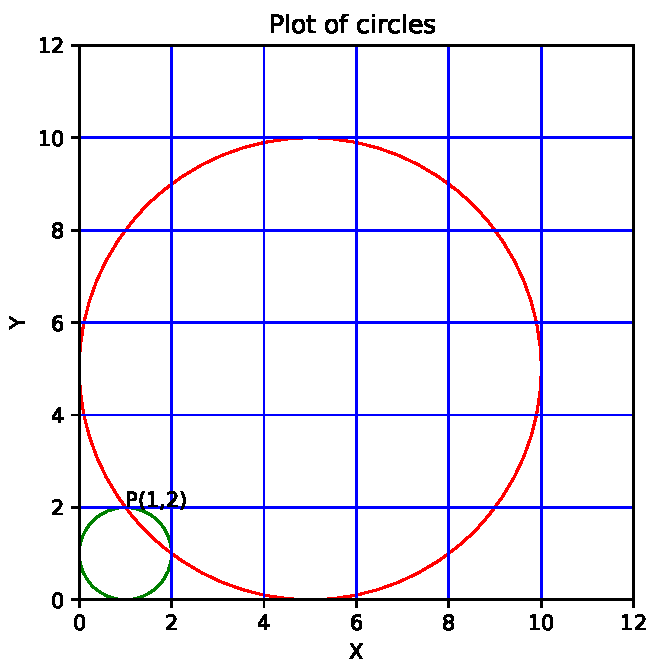
\includegraphics[width=.50 \textwidth, height=.30\textheight]{figure1.pdf}	
	\caption{Two circles passes through the point}
	\label{fig1}	
\end{figure}

\begin{align}
 \implies r  =  \frac{r^2 - 5}{2 \left(r - 3\right)} 
\end{align}


\begin{align}
\implies r^2 - 6r +5 = 0
\end{align}


\begin{align}
\implies \left( r -1\right) \left( r- 5\right) = 0
\end{align}

\begin{align}
\implies r = 1, r = 5.
\end{align}

Hence,
\begin{align}
\vec{O_1} = \myvec{5 \\ 5 \\} \text{and,}  \vec{O_2} = \myvec{1 \\ 1 \\}
\end{align}

Hence equation of circles are :
\begin{align}
\norm{\vec{x} - \myvec{5 \\ 5 \\}} = 5
\end{align}
And,
\begin{align}
\norm{\vec{x} - \myvec{1 \\ 1 \\}} = 1
\end{align}

\end{document}
